\chapterauthor{Andreas Kölbl}

\chapter{Arbeitspaket Motor}
Die Analyse, Implementierung, Test und Integration, sowie die Verkabelung der H-Brücke mit Unterst\"utzung von Herrn Brunner f\"ur Hardware-relevante Problemstellungen war Aufgabe von Herrn Kölbl. Die Drehzahl des Motors soll gesteuert werden können.

\section{Analysephase}
Aus der Projektspezifikation ergibt sich, dass sich der Motor in zwei Richtungen drehen soll. Auch soll die Drehzahl des Motors einstellbar sein. Um das zu erreichen, ist die H-Brücke manuell oder mit der Software InstaSPIN zu bedienen. Der Motor soll durch den Microcontroller kommutiert werden. Hierfür soll das POSIF-Interface verwendet werden, um schnellere Schaltzyklen gewährleisten zu können. Auch sind bereits dort Abläufe zur Kommutierung einprogrammiert. Das vermeidet redundanten Coden, wenn man auf einen anderen Infineon-Chip wechselt.

\subsection{Verkabelung Motor}
\begin{figure}
    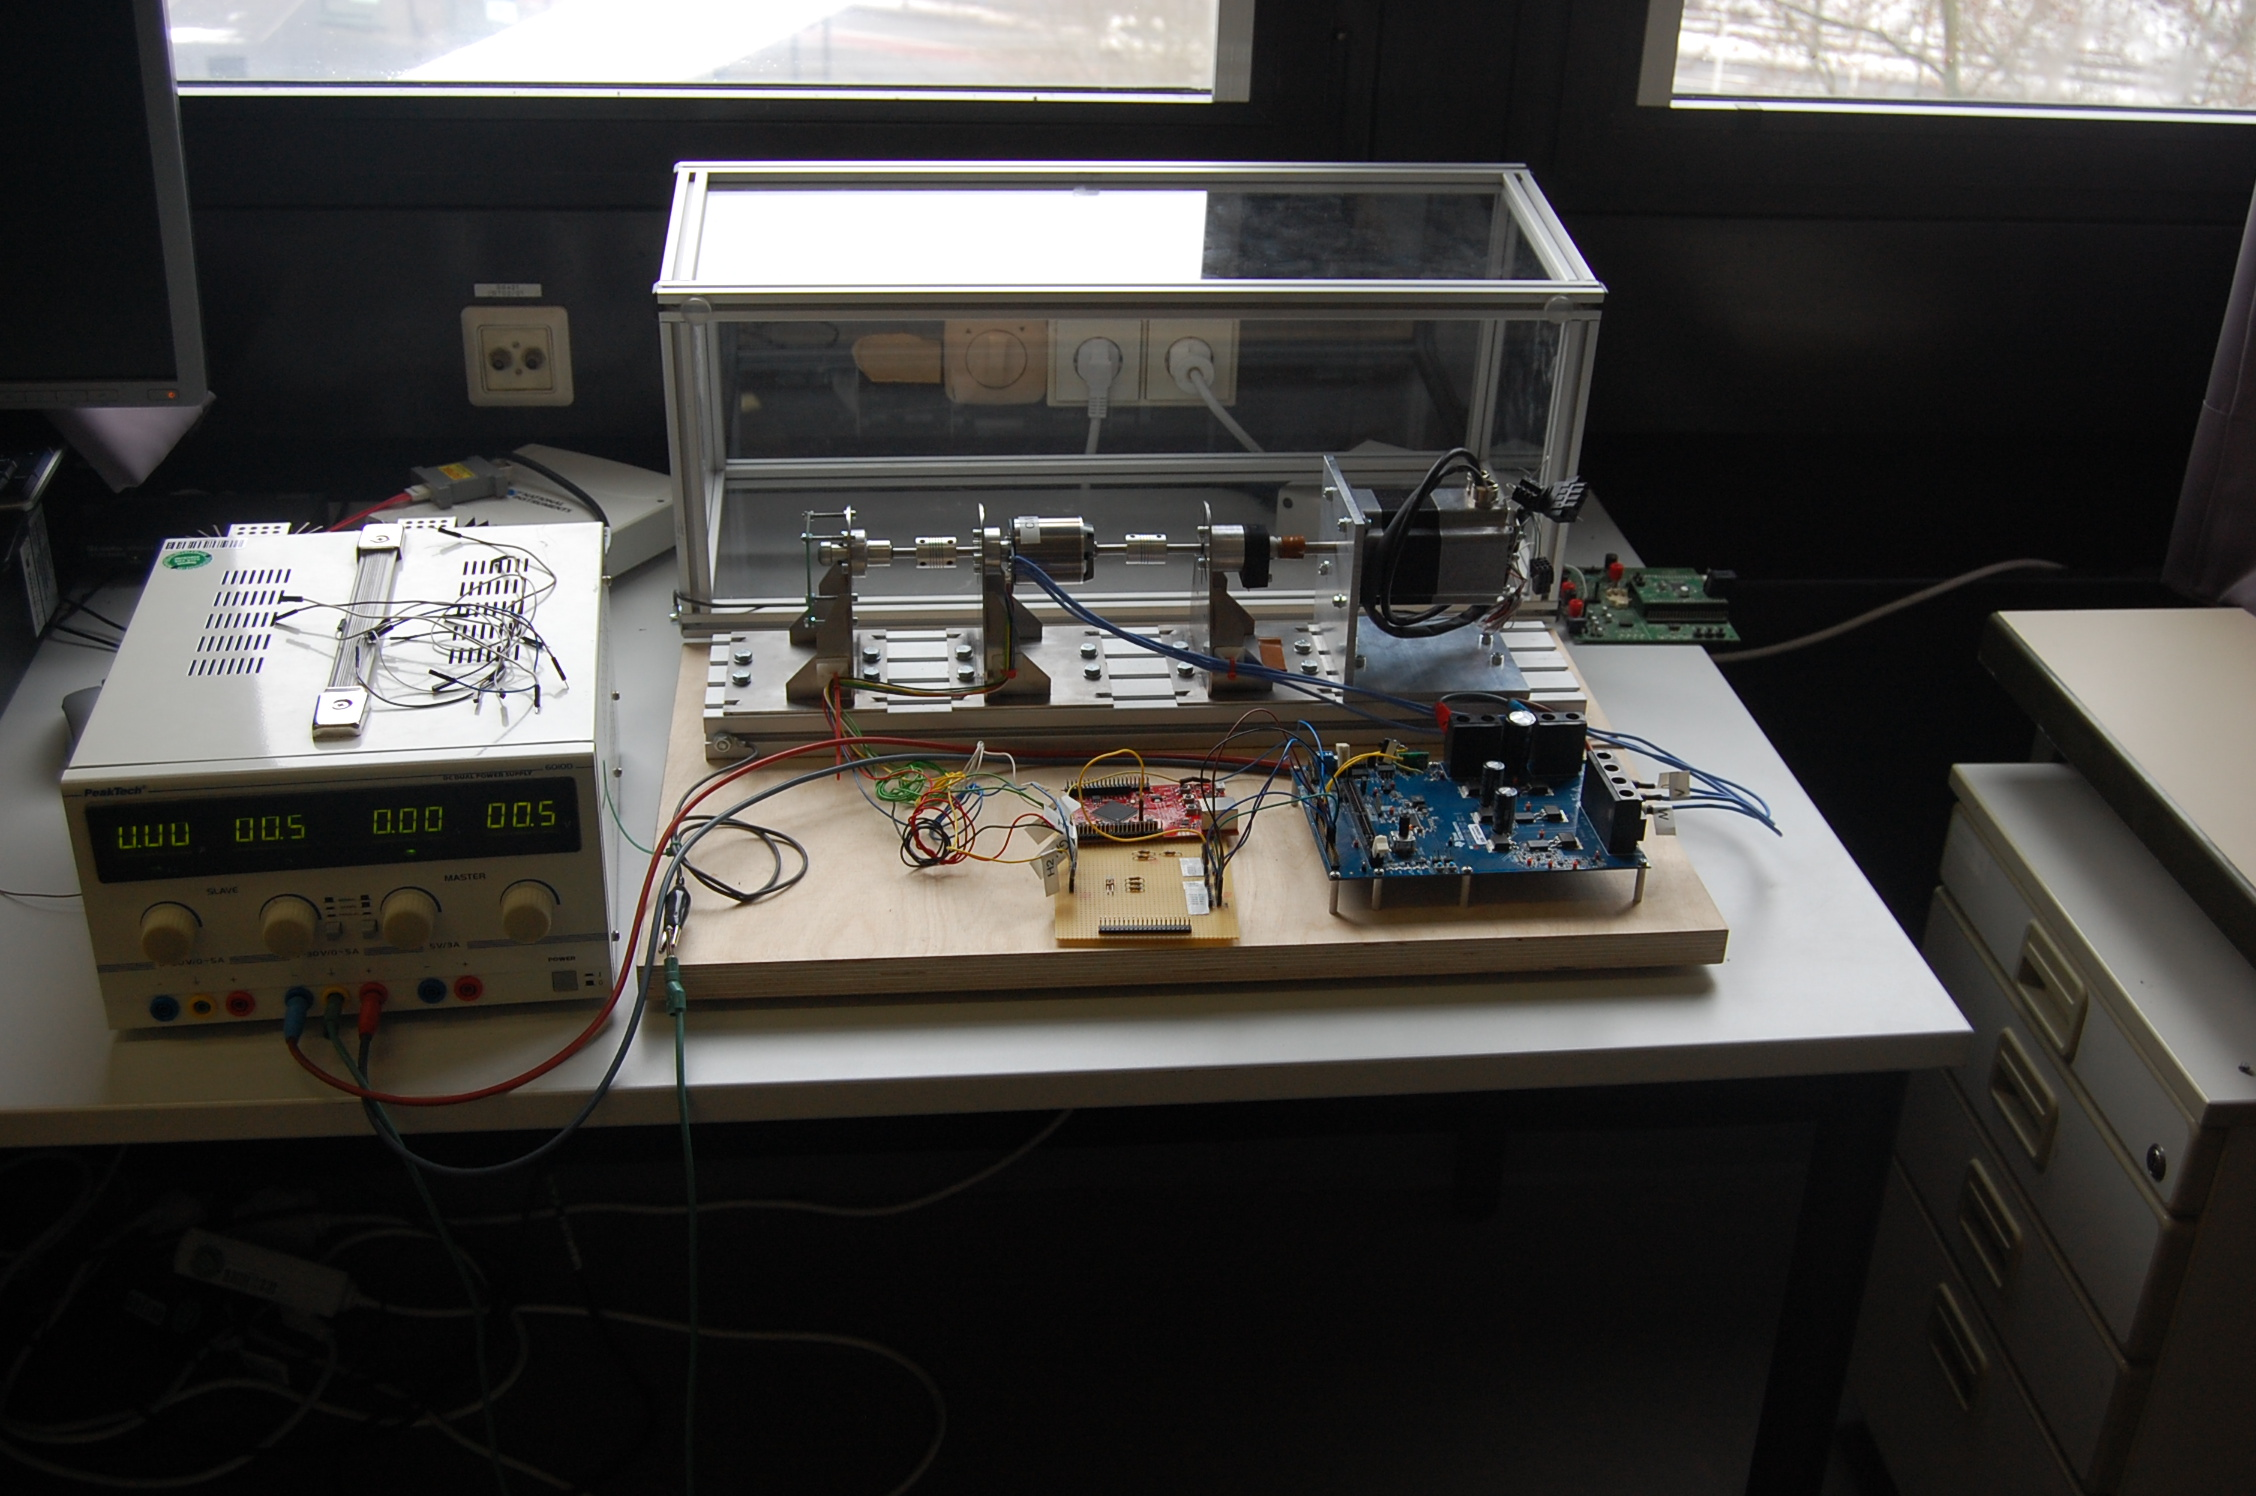
\includegraphics[width=\textwidth]{motor/MotorWiring.JPG}
    \caption{Verkabelung des Motors}
    \label{fig:MotorWiring}
\end{figure}

Die in der Abbildung \ref{fig:MotorWiring} zu sehende H-Brücke ist mit einem Netzteil (im ausgeschaltetem Zustand) und dem Motor verbunden. Es wäre auch ein Netzteil mit einer höheren Ausgangsspannung einsetzbar, da die H-Brücke bis zu 60V Gleichspannung betrieben werden kann. Das Erdungskabel zum Netzteil ist mit dem Motor verbunden. \\
Die H-Brücke wurde außerdem noch mit der Adapterplatine gemäß dem Schaltplan verbunden. In dem Ausschnitt \ref{fig:TIWiring} ist der PIN-Header "External Control" zu sehen, der zur manuellen Kommutierung benutzt wird. Dabei sind die drei Phasen U, V und W mit deren jeweiligen High- und Low-Anschluss als PWM\_AH, PWM\_AL, PWM\_BH, PWM\_BL, PWM\_CH und PWM\_CL beschrieben. Diese sind mit dem Mikrocontroller zu verbinden. Dabei muss man darauf zu achten, dass die jeweiligen Pins auf dem Controller für die Capture-Compare Units verwendet werden können \cite{InfineonTechnologies2016}.
\begin{figure}
    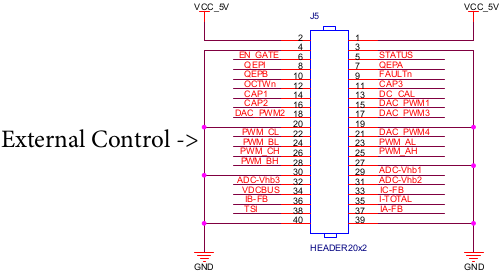
\includegraphics[width=0.66\textwidth]{motor/TI_Wiring.png}
    \caption{H-Brücke 40 Pin-Header}
    \quelle \cite{Instruments2014}
    \label{fig:TIWiring}
\end{figure}
Der Motor muss mit den Stromausgängen U, V und W verbunden werden. Die Kabel wurden für diesen Zweck beschriftet. \\

\subsection{BLDC-Motor}
Den Brushless DC-Motor zu verwenden bringt Vor- und Nachteile mit sich.

Der allgemeine Vorteil von Bürstenlosen Motoren liegt darin, dass es keine Verschleißteile gibt.
Hingegen müssen bei klassischen Gleichstrommotoren mit Bürsten diese ersetzt werden sobald sie verbraucht oder zerstört sind. Im Idealfall werden auch keine störenden Induktionsspannungen durch die Stromwendung erzeugt \cite{Babiel2014}. Der bürstenlose Motor läuft sehr leise und lässt sich sehr genau von ganz langsam (nicht alle) bis ganz schnell elektronisch regeln. Dazu hat er erheblich mehr Kraft bei gleichen Abmessungen oder einen geringeren Stromverbrauch mit weniger Verlustleistung. \\
Der Nachteil des BLDC-Motors ist, dass der Motor nicht stehen bleibt, wenn die Spannung weg ist. Er muss gezielt abgebremst und gestoppt werden.
Durch den deutlich höheren Preis sollten diese bürstenlosen DC Motoren nur in anspruchsvollen Geräten eingesetzt werden.
Die Auswahlkriterien für die bürstenlosen Gleichstromservomotoren sind meist "extrem präzise stufenlose Geschwindigkeit" bei sich stetig ändernder Last im geschlossenen Regelkreis mit Prozessorsteuerung.

\subsection{TI InstaSPIN}
Die von Texas Instruments gelieferte H-Brücke bietet zusätzlich zum manuellen Ansteuern eines Motors noch die Möglichkeit, diesen über das Programm InstaSPIN anzusteuern. Hierfür ist eine lizensierte Steuerkarte enthalten, die mit einer Testlizenz von 30 Tagen geliefert wurde. \\
Eine Ansteuerung über eine virtualisiertes Windows-Betriebssystem war nicht möglich, da Linux als Betriebssystem nicht unterstützt wird. Dieses Programm führt eine Ansteuerung des Motors ohne Hall-Sensoren durch. Hierbei wird lediglich der Spannungsabfall am Stromausgang durch einen ADC-Converter gemessen und den Messwerten entsprechend kommutiert. Über den Drehregler in Abbildung \ref{fig:InstaSPIN} lässt sich die Drehzahl des Motors beeinflussen.
\begin{figure}
    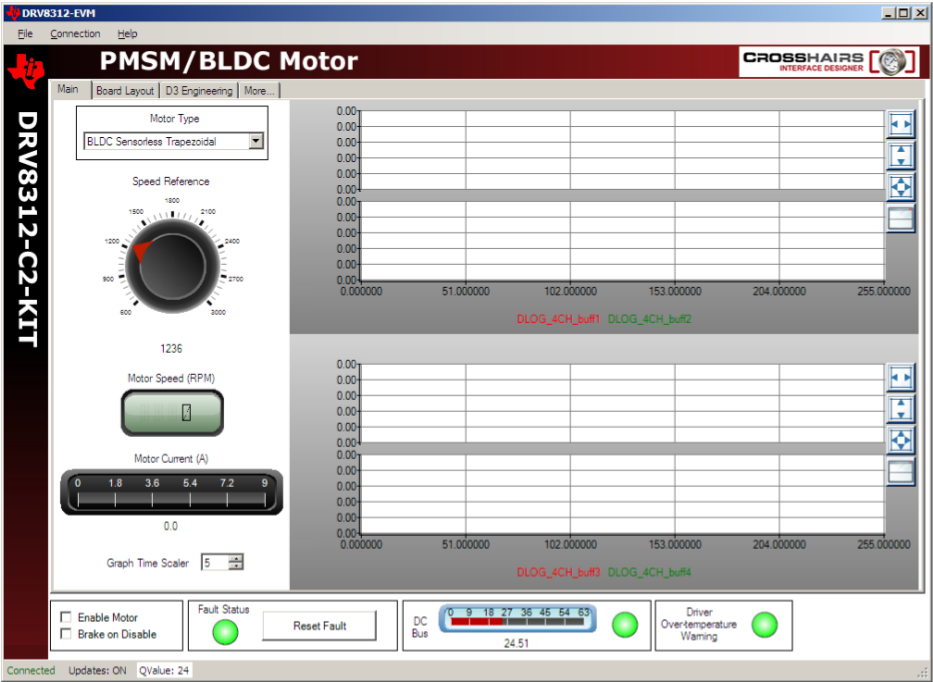
\includegraphics[width=\textwidth]{motor/InstaSPIN}
    \caption{Texas Instruments InstaSPIN}
    \quelle \cite{Instruments2011}
    \label{fig:InstaSPIN}
\end{figure}
\section{Implementierung}
\subsection{POSIF}
\subsubsection{Zweck von POSIF}
Da Software als solches in der Erstellung und Pflege teurer wird und Hardwarekosten stetig sinken, ist ein Trend erkennbar, Software direkt als Hardware zu implementieren. Das Ergebnis sind bessere Schaltgeschwindigkeiten und weniger Kosten durch Programmierung und Wartung von Software. So erreicht man durch die besseren Schaltgeschwindigkeiten neue Rekorde, wie bspw. den \emph{Rubik's Cube} am schnellsten zu lösen \cite{POSIF2016}.

\subsubsection{Zuweisung im Multi-Channel Mode}
In Abbildung \ref{fig:interconnects} wird die interne Verschaltung des POSIF-Interfaces mit den jeweiligen Capture-Compare Units dargestellt. Die Capture-Compare Units geben das PWM-Signal auf deren jeweilig zugewiesenen Ausgängen aus, sobald ein neues \emph{Correct Hall Event} aufgetreten ist. Wie diese Zuweisung auszusehen hat, kann leider nur durch das lesen vieler Dokumente die auf der Website von Infineon bei den Chips der Serie XMC1000/XMC4000 erahnt werden. Letztlich gibt der Code vom XMC44xx-Chip von Infineon ein vorbildliches Beispiel, wie das POSIF-Interface zu implementieren ist. Es ist notwendig, die Variablen, die in Abbildung \ref{fig:interconnects} dargestellt sind, den entsprechenden Ausgängen zuzuweisen.  Leider wurde dieses Beispiel eines anderen Chips erst in einer sehr späten Projektphase entdeckt. Deswegen ist im Beispielcode das POSIF-Interface lediglich dazu da, Hall-Events weiterzuleiten. Je nach Hall-Event werden die Ausgänge zum Schalten der Motoren mit voller Leistung angetrieben.
\begin{figure}
    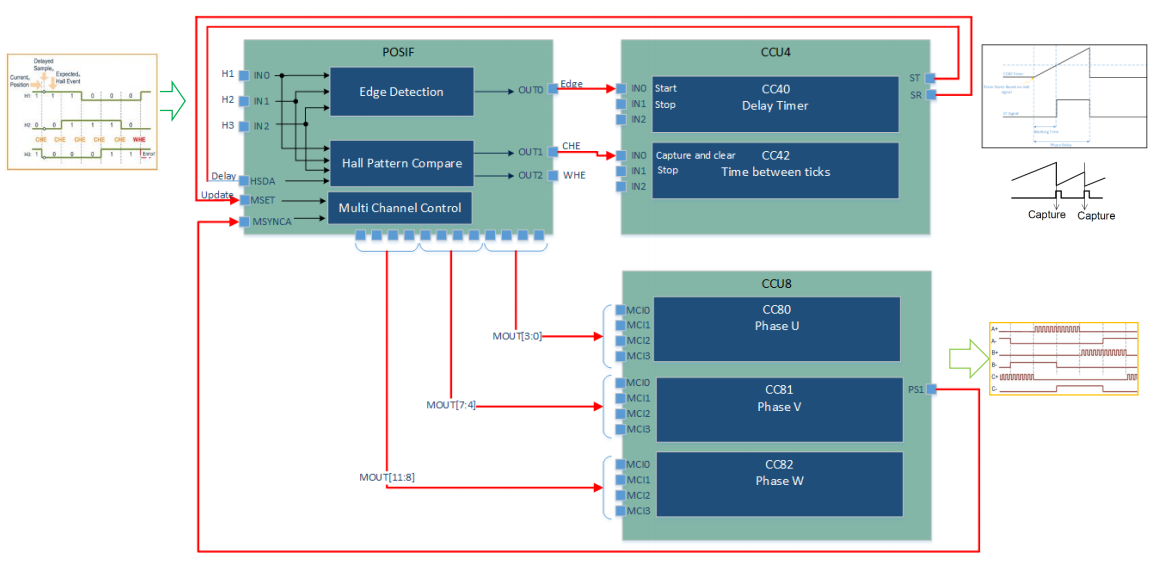
\includegraphics[width=\textwidth]{motor/interconnects}
    \caption{Verbindungen des Patterns zum Ausgang einer CCU Slice}
     \quelle {Infineon}
    \label{fig:interconnects}
\end{figure}

\section{Ausblick}
Der Code zur Steuerung und Regelung des Motors befindet sich momentan noch in den Anfängen. Bei der aktuellen Bearbeitungslage ist eine vollständige Fertigstellung nicht absehbar. \\
Basierend auf der Ideensammlung aus der Analysephase wäre eine mögliche Erweiterung dieses Arbeitspaketes die Portierung des Codes auf eine andere Hardwareplattform ohne POSIF-Interface. Das hätte eine Neuimplementierung der Steuerung zur Folge. \\
Der Beispielcode des POSIF-Interfaces, welches alle Features des POSIF-Interfaces nutzt wäre ein sinnvoller Ansatz, um eine Portierung vom XMC44xx-Chip zum XMC4800 vorzunehmen. Somit können alle Vorteile des POSIF-Interfaces ausgenutzt werden. \\
Die Verkabelung muss noch gesichert werden. Die H-Brücke soll außerdem während des Betriebs durch eingriffe in die Elektronik geschützt werden, da an den auf der H-Brücke verbauten Kondensatoren sehr hohe Ströme auftreten können. 

